\documentclass[12pt,a4paper]{article}
\usepackage[T1]{fontenc}
\usepackage{amsmath,amssymb,mathrsfs,tikz,times,pifont}
\usepackage{enumitem}
\usepackage{multicol}
\usepackage{lmodern}
\usetikzlibrary{trees}
\newcommand\circitem[1]{%
\tikz[baseline=(char.base)]{
\node[circle,draw=gray, fill=red!55,
minimum size=1.2em,inner sep=0] (char) {#1};}}
\newcommand\boxitem[1]{%
\tikz[baseline=(char.base)]{
\node[fill=cyan,
minimum size=1.2em,inner sep=0] (char) {#1};}}
\setlist[enumerate,1]{label=\protect\circitem{\arabic*}}
\setlist[enumerate,2]{label=\protect\boxitem{\alph*}}
%%%::::::by chnini ameur :::::::%%%
\everymath{\displaystyle}
\usepackage[left=1cm,right=1cm,top=1cm,bottom=1.7cm]{geometry}
\usepackage[colorlinks=true, linkcolor=blue, urlcolor=blue, citecolor=blue]{hyperref}
\usepackage{array,multirow}
\usepackage[most]{tcolorbox}
\usepackage{varwidth}
\usepackage{float} %pour utiliser l'option [H] qui force l'image à apparaître exactement à l'endroit où elle est placée dans le code.
\tcbuselibrary{skins,hooks}
\usetikzlibrary{patterns}
%%%::::::by chnini ameur :::::::%%%
\newtcolorbox{exa}[2][]{enhanced,breakable,before skip=2mm,after skip=5mm,
colback=yellow!20!white,colframe=black!20!blue,boxrule=0.5mm,
attach boxed title to top left ={xshift=0.6cm,yshift*=1mm-\tcboxedtitleheight},
fonttitle=\bfseries,
title={#2},#1,
% varwidth boxed title*=-3cm,
boxed title style={frame code={
\path[fill=tcbcolback!30!black]
([yshift=-1mm,xshift=-1mm]frame.north west)
arc[start angle=0,end angle=180,radius=1mm]
([yshift=-1mm,xshift=1mm]frame.north east)
arc[start angle=180,end angle=0,radius=1mm];
\path[left color=tcbcolback!60!black,right color = tcbcolback!60!black,
middle color = tcbcolback!80!black]
([xshift=-2mm]frame.north west) -- ([xshift=2mm]frame.north east)
[rounded corners=1mm]-- ([xshift=1mm,yshift=-1mm]frame.north east)
-- (frame.south east) -- (frame.south west)
-- ([xshift=-1mm,yshift=-1mm]frame.north west)
[sharp corners]-- cycle;
},interior engine=empty,
},interior style={top color=yellow!5}}
%%%%%%%%%%%%%%%%%%%%%%%
\usepackage{fancyhdr}
\usepackage{eso-pic}         % Pour ajouter des éléments en arrière-plan
% Commande pour ajouter du texte en arrière-plan
\usepackage{tkz-tab}
\usepackage{tikz}
\usetikzlibrary{calc, intersections}
\usepackage[siunitx, european, RPvoltages]{circuitikz}
\AddToShipoutPicture{
    \AtTextCenter{%
        \makebox[0pt]{\rotatebox{80}{\textcolor[gray]{0.7}{\fontsize{5cm}{5cm}\selectfont PGB}}}
    }
}
\usepackage{lastpage}
\fancyhf{}
\pagestyle{fancy}
\renewcommand{\footrulewidth}{1pt}
\renewcommand{\headrulewidth}{0pt}
\renewcommand{\footruleskip}{10pt}
\fancyfoot[R]{
\color{blue}\ding{45}\ \textbf{2026}
}
\fancyfoot[L]{
\color{blue}\ding{45}\ \textbf{Prof:M. BA}
}
\cfoot{\bf
\thepage /
\pageref{LastPage}}
% Création du compteur pour les exercices
\newcounter{exercice}
\renewcommand{\theexercice}{\arabic{exercice}}  % Définit l'affichage du compteur en chiffres arabes

% Définir la commande \exo
\newcommand{\exo}{\refstepcounter{exercice}\textbf{Exercice \theexercice} }
\begin{document}
\renewcommand{\arraystretch}{1.5}
\renewcommand{\arrayrulewidth}{1.2pt}
\begin{tikzpicture}[overlay,remember picture]
    \node[draw=blue,line width=1.2pt,fill=purple,text=blue,inner sep=3mm,rounded corners,pattern=dots]at ([yshift=-2.5cm]current page.north) {\begingroup\setlength{\fboxsep}{0pt}\colorbox{white}{\begin{tabular}{|*1{>{\centering \arraybackslash}p{0.28\textwidth}} |*2{>{\centering \arraybackslash}p{0.2\textwidth}|} *1{>{\centering \arraybackslash}p{0.19\textwidth}|} }
                \hline
                \multicolumn{3}{|c|}{$\diamond$$\diamond$$\diamond$\ \textbf{Lycée de Dindéfélo}\ $\diamond$$\diamond$$\diamond$ } & \textbf{A.S. : 2026/2027}                                              \\ \hline
                \textbf{Matière: Mathématiques}                                                                                    & \textbf{Niveau : 3}\textbf{M1} & \textbf{Date: 20/11/2026} & \textbf{} \\ \hline
                \multicolumn{4}{|c|}{\parbox[c]{10cm}{\begin{center}
                                                                  \textbf{{\Large\sffamily Théorème de Thalès}}
                                                              \end{center}}}                                                                                                        \\ \hline
            \end{tabular}}\endgroup};
\end{tikzpicture}
\vspace{3cm}
\begin{multicols}{2}
\setlength{\columnseprule}{0.1mm} % La largeur de la ligne verticale entre les colonnes
\fbox{\textbf{\exo}} \textbf{4pts}

\end{multicols}
On donne $OA = 4\text{ cm}$ ; $OB = 5\text{ cm}$ ; $OJ = 12\text{ cm}$ et $OK = 15\text{ cm}$.

\begin{center}
\begin{tikzpicture}[scale=0.55]
    % Définition des coordonnées à l'échelle (1 unité = 1 cm)
    % Intersection O à l'origine
    \coordinate (O) at (0,0);
    % Droite (AJ) avec un angle de -30 degrés
    \coordinate (A) at (150:4);
    \coordinate (J) at (-30:12);
    % Droite (BK) avec un angle de 15 degrés
    \coordinate (B) at (-165:5);
    \coordinate (K) at (15:15);

    % Tracé des droites (AB) et (KJ) prolongées
    \draw[thin] ($(B)!-0.45!(A)$) -- ($(A)!-0.45!(B)$);
    \draw[thin] ($(J)!-0.2!(K)$) -- ($(K)!-0.2!(J)$);

    % Tracé des segments sécants [AJ] et [BK]
    \draw[thick] (A) -- (J);
    \draw[thick] (B) -- (K);

    % Marquage des points
    \foreach \p in {A,B,J,K} {
        \filldraw[fill=white, draw=black] (\p) circle (2.2pt);
    }

    % Étiquettes des points
    \node[above left, font=\bfseries] at (A) {A};
    \node[above left, font=\bfseries] at (B) {B};
    \node[below=5pt, font=\bfseries] at (O) {O};
    \node[right=4pt, font=\bfseries] at (J) {J};
    \node[right=4pt, font=\bfseries] at (K) {K};
\end{tikzpicture}
\end{center}
\begin{enumerate}
\item Les droites $(AB)$ et $(KJ)$ sont-elles parallèles ? Justifie ta réponse. \hfill \textbf{(2 pts)}
\item On donne aussi $AB = 3\text{ cm}$, calcule $KJ$. \hfill \textbf{(2 pts)}
\end{enumerate}

\fbox{\textbf{\exo}}  \textbf{6,5 pts}

\begin{enumerate}
\item Dans la figure ci-dessous $ABCD$ est un trapèze. La droite $(EF)$ qui passe par $G$ est parallèle aux bases $(AB)$ et $(DC)$.
\begin{center}
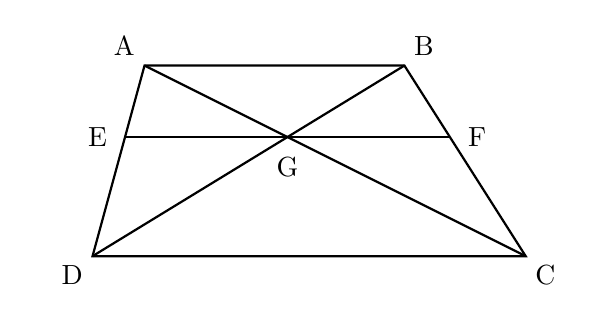
\begin{tikzpicture}[scale=1.1]
    % Sommets du trapèze ABCD
    \coordinate (D) at (0,0);
    \coordinate (C) at (5,0);
    \coordinate (A) at (0.6,2.2);
    \coordinate (B) at (3.6,2.2);

    % Tracé des côtés du trapèze
    \draw[thick] (A) -- (B) -- (C) -- (D) -- cycle;

    % Tracé des diagonales et calcul de leur intersection G
    \draw[thick, name path=AC] (A) -- (C);
    \draw[thick, name path=BD] (B) -- (D);
    \path[name intersections={of=AC and BD, by=G}];

    % Droite horizontale passant par G coupant [AD] en E et [BC] en F
    \path[name path=AD] (A) -- (D);
    \path[name path=BC] (B) -- (C);
    \path[name path=horiz] ($(G)-(3,0)$) -- ($(G)+(3,0)$);
    \path[name intersections={of=AD and horiz, by=E}];
    \path[name intersections={of=BC and horiz, by=F}];

    % Tracé du segment [EF]
    \draw[thick] (E) -- (F);

    % Étiquettes des points
    \node[above left] at (A) {A};
    \node[above right] at (B) {B};
    \node[below right] at (C) {C};
    \node[below left] at (D) {D};
    \node[left=3pt] at (E) {E};
    \node[right=3pt] at (F) {F};
    \node[below=4pt] at (G) {G};
\end{tikzpicture}
\end{center}

En utilisant la figure, donnne trois couples ( paires) de triangles en position de Thales. \quad (1,5pts)

\item EFG est un triangle rectangle en E tels que EF=6cm et EG=8cm.

\begin{enumerate}
\item Fais une figure que tu complèteras au fur et à mesure. \hspace{3cm} \textbf{(1pt)}\\
\item Calcule FG. \hspace{8.8cm} \textbf{(1pt)}\\
\item Place un point M sur [EF] tel que EM=2,4cm. La parallèle à (FG) passant par M coupe (EG) en N. Calcules EN et MN. \hspace{2.5cm} \textbf{(2pts)}\\
\item Marque un point O sur [MN] tel que MO=10cm.\\
Les droites (EM) et (OG) sont-elles parallèles ? \hspace{3.2cm} \textbf{(1point)}
\end{enumerate}
\end{enumerate}

\end{document}